\chapter{Wyniki eksperymentów}
\thispagestyle{chapterBeginStyle}

W tym rozdziale przyjrzymy się wynikom przeprowadzonych eksperymentów dla omawianych wcześniej algorytmów i ich ulepszeń. Na początku rozważymy algorytm \texttt{MinCount} - porównamy podejście naiwne, ulepszenie zaproponowane w rozdziale 2 oraz metodę \textit{estymatora ważonego} dla tego algorytmu. Następnie dla algorytmu \texttt{HyperLogLog}, skupimy się głównie na operacji przekroju - porównamy podejście naiwne, korzystające z indeksu \textit{Jaccarda} i metodę estymatora \textit{ważonego} dla tegoż algorytmu. Na koniec porównamy efektywność obu algorytmów w kontekście operacji teoriomnogościowych i postaramy się określić które z nich sprawdzą się najefektywniej w praktyce. Eksperymenty przeprowadzone w tym rozdziale badają dokładność algorytmów na przestrzeni różnych indeksów \textit{Jaccarda}. Dokładność algorytmu mierzymy przez $\frac{\hat{n}}{n}$, czyli stosunek liczności zbioru wyznaczonej przez estymator do prawdziwej liczności zbioru. We wszystkich eksperymentach dla algorytmu \texttt{MinCount}, ustaliliśmy parametr $k = 100$, czyli szkice przetrzymywały 100 najmniejszych haszy.

\section{Wyniki dla algorytmu MinCount}
Na początek przedstawiamy wyniki dla trzech metod estymacji dla algorytmu \texttt{MinCount}:
\begin{enumerate}
	\item metoda naiwna (z \textit{zasady włączeń i wyłączeń})
	\item ulepszenie zaproponowane w rozdziale 2
	\item metoda \textit{estymatora ważonego}
\end{enumerate}

Wykresy \ref{fig:KMV_2sets_inter} oraz \ref{fig:KMV_2sets_sum} przedstawiają wyniki eksperymentów dla sum i przekrojów dwóch zbiorów.

\begin{figure}[h!]
    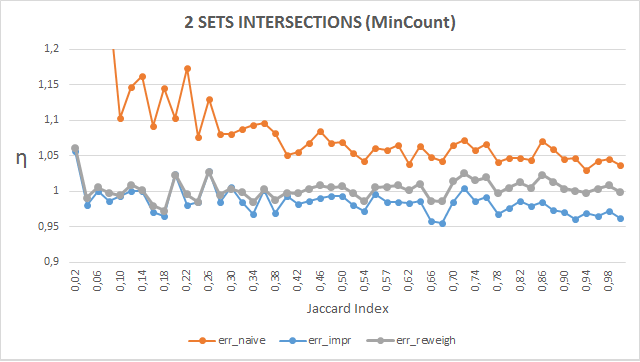
\includegraphics[width=0.6\textwidth]{KMV_2_sets_inter.png}
    \centering
    \caption{Porównanie metod dla przekrojów 2 zbiorów}
    \label{fig:KMV_2sets_inter}
\end{figure}

\begin{figure}[h!]
    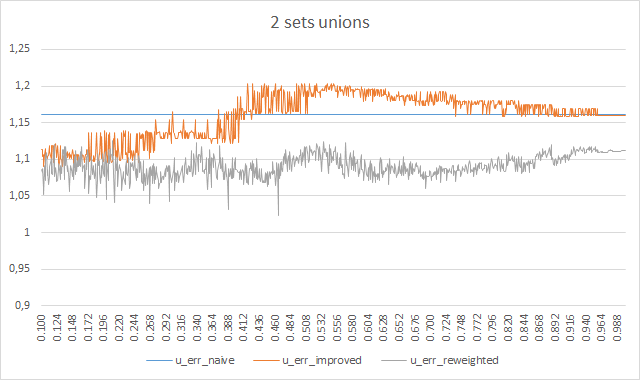
\includegraphics[width=0.6\textwidth]{KMV_2_sets_sum.png}
    \centering
    \caption{Porównanie metod dla sumy 2 zbiorów}
    \label{fig:KMV_2sets_sum}
\end{figure}

Zauważmy, że dla operacji sumy - praktycznie na całym przedziale indeksów \textit{Jaccarda} zbiorów - najmniejszy błąd posiada metoda \textit{estymatora ważonego}. W przypadku przekroju, dla indeksów \textit{Jaccarda} większych niż ok. $0.20$ najlepiej wypada estymacja przy użyciu naiwnej metody wykorzystującej zasadę \textit{włączeń i wyłączeń} - pamiętajmy jednak, że jest to przypadek z użyciem tylko dwóch zbiorów, gdzie wzór ten jest jeszcze stosunkowo nieskomplikowany, oraz że ta metoda estymacji nie prowadzi do utworzenia nowego szkicu reprezentującego przekrój, a więc nie możemy wykonać kolejnych operacji z jego użyciem. W przypadku pozostałych metod dla przekroju znowu widzimy zysk na dokładności poprzez użycie \textit{estymatora ważonego}, nawet dla wartości indeksów \textit{Jaccarda}, dla których metoda naiwna posiadała bardzo duży błąd oraz anomalie (ujemne estymaty).

Na kolejnych wykresach, zestawiliśmy wyniki dla sum i przekrojów większej liczby zbiorów. Wykonaliśmy eksperymenty dla 100 oraz 1000 zbiorów, porównując metody $2.$ oraz $3.$ Metodę naiwną pominęliśmy ze względu na jej znaczące wady wspomniane w poprzednim akapicie. Dla większej liczby zbiorów widać coraz większą efektywność metody \textit{estymatora ważonego} la indeksów \textit{Jaccarda} wiekszych niż ok. $3.50$. Wraz z wzrostem liczby zbiorów biorących udział w operacji - wzrasta liczba estymatorów składowych, a więc liczba ważonych składników - przez co zauważyć możemy efekt \textit{ważenia}, zmniejszający błąd względem pojedynczego estymatora.

\begin{figure}[h!]
    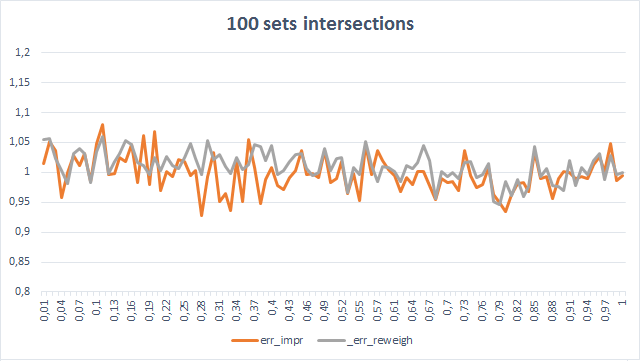
\includegraphics[width=0.6\textwidth]{KMV_100_sets_inter.png}
    \centering
    \caption{Porównanie metod dla przekroju 100 zbiorów}
    \label{fig:KMV_1000sets_inter}
\end{figure}

\begin{figure}[h!]
    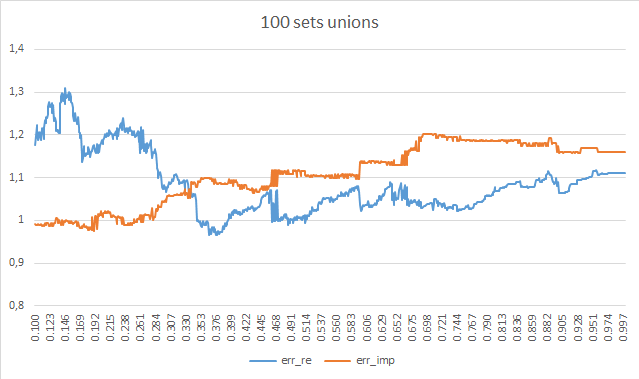
\includegraphics[width=0.6\textwidth]{KMV_100_sets_sum.png}
    \centering
    \caption{Porównanie metod dla sumy 100 zbiorów}
    \label{fig:KMV_100sets_sum}
\end{figure}

\begin{figure}[h!]
    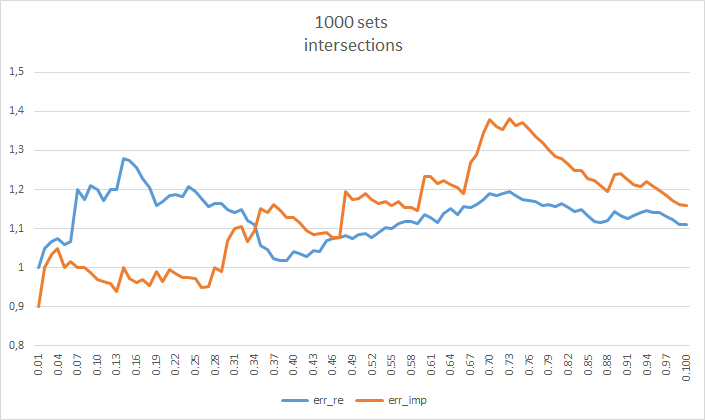
\includegraphics[width=0.6\textwidth]{KMV_1000_sets_inter.png}
    \centering
    \caption{Porównanie metod dla przekroju 1000 zbiorów}
    \label{fig:KMV_100sets_inter}
\end{figure}

\begin{figure}[h!]
    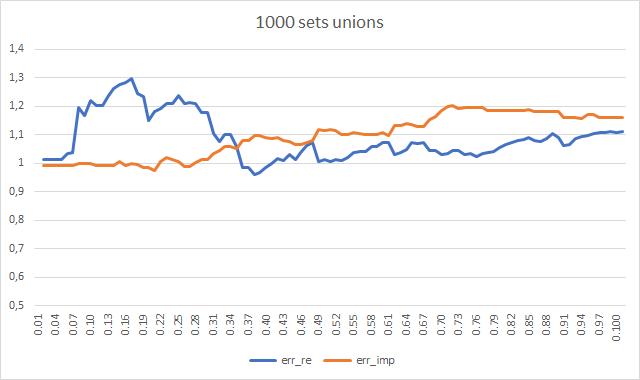
\includegraphics[width=0.6\textwidth]{KMV_1000_sets_sum.png}
    \centering
    \caption{Porównanie metod dla sumy 1000 zbiorów}
    \label{fig:KMV_1000sets_sum}
\end{figure}

Ostatnimi eksperymentami przeprowadzonymi dla algorytmu \texttt{MinCount} było sprawdzenie metody \textit{estymatora ważonego} dla różnicy zbiorów, omówionej w rozdziale $4.4$. Na wykresie \ref{fig:KMV_2_sets_diff} przedstawiamy wyniki dla różnicy dwóch zbiorów, porównując podejście naiwne oraz podejście wykorzystujące \textit{estymator ważony}.

\begin{figure}[h!]
    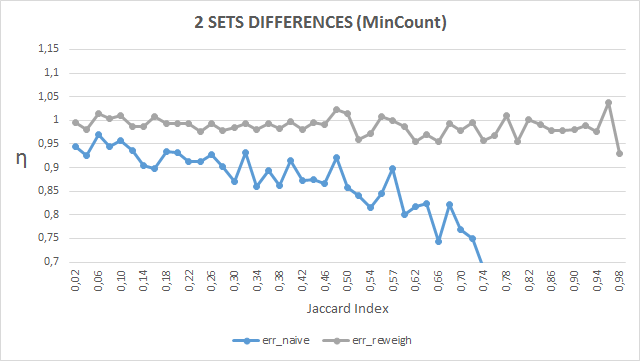
\includegraphics[width=0.6\textwidth]{KMV_2_sets_diff.png}
    \centering
    \caption{Porównanie metod dla różnicy 2 zbiorów}
    \label{fig:KMV_2_sets_diff}
\end{figure}

\newpage
\section{Wyniki dla algorytmu HyperLogLog}
W tym podrozdziale przedstawimy wyniki dla algorytmu \texttt{HyperLogLog}. Zestawiliśmy ze sobą dwie metody:
\begin{enumerate}
	\item metoda naiwna z użyciem indeksu \textit{Jaccarda} (wzór $(2.19)$)
	\item metoda \textit{estymatora ważonego}
\end{enumerate}
Obydwie metody korzystają z pomocniczej struktury dla każdego ze szkiców, przechowującej $k$ najmniejszych wartości (czyli zasadniczo z podstawowej wersji szkicu \texttt{MinCount}), pozwalającej na estymację indeksu \textit{Jaccarda} \cite{adroll}, potrzebnego zarówno do estymacji metoda naiwna jak i metoda \textit{estymatora ważonego}. W przeprowadzanych eksperymentach ustaliliśmy parametry $k = 80$ oraz $b = 8$.

Na wykresach \ref{fig:HLL_100_sets_sum} oraz \ref{fig:HLL_100_sets_inter} przedstawiamy porównanie powyższych metod w kontekście operacji sumy oraz przekroju. Eksperymenty przeprowadziliśmy dla 100 zbiorów.

\begin{figure}[h!]
    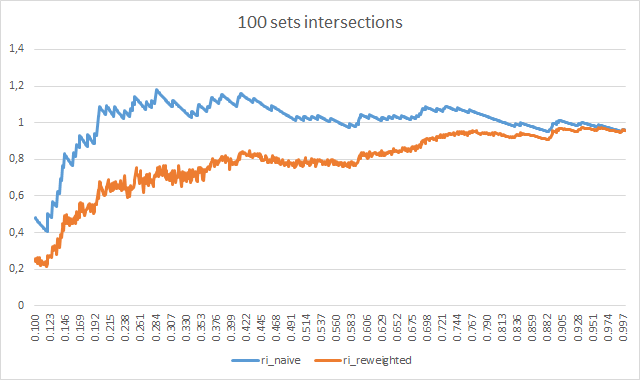
\includegraphics[width=0.6\textwidth]{HLL_100_sets_inter.png}
    \centering
    \caption{Porównanie metod dla przekroju 100 zbiorów}
    \label{fig:HLL_100_sets_inter}
\end{figure}

\begin{figure}[h!]
    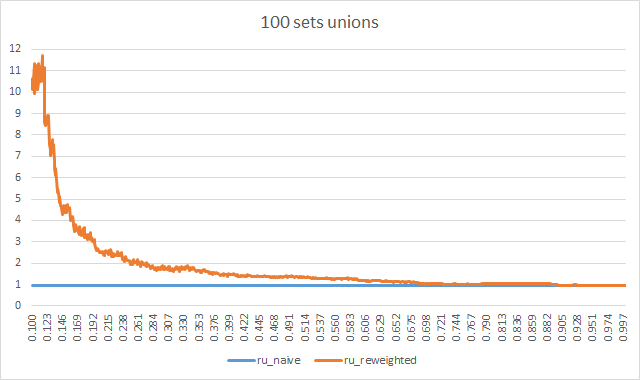
\includegraphics[width=0.6\textwidth]{HLL_100_sets_sum.png}
    \centering
    \caption{Porównanie metod dla sumy 100 zbiorów}
    \label{fig:HLL_100_sets_sum}
\end{figure}

Wnioski wynikające z tych eksperymentów sugerują, że metoda \textit{estymatora ważonego} w kontekście algorytmu \texttt{HyperLogLog} niestety nie dorównuje pod względem dokładności podejściu naiwnemu. W przypadku sumy jest to dosyć oczywiste, ponieważ jak wspominaliśmy w rozdziale 2 - \texttt{HyperLogLog} posiada naturalną operację sumy, która posiada stały i niewielki błąd, niezależnie od podobieństwa sumowanych zbiorów. W przypadku operacji przekroju metoda naiwna wykorzystująca indeks \textit{Jaccarda} i wzór $(2.19)$ posiada mniejszy błąd niż estymacja z użyciem \textit{estymatora ważonego}. Zauważmy że obie metody wykorzystują tyle samo pamięci, bowiem obie wymagają dodatkowej struktury pozwalającej na estymację indeksu \textit{Jaccarda} przy wykorzystaniu algorytmu \texttt{MinHash}.